\section{Messprotokoll}
\begin{figure}[h!]
    \centering
    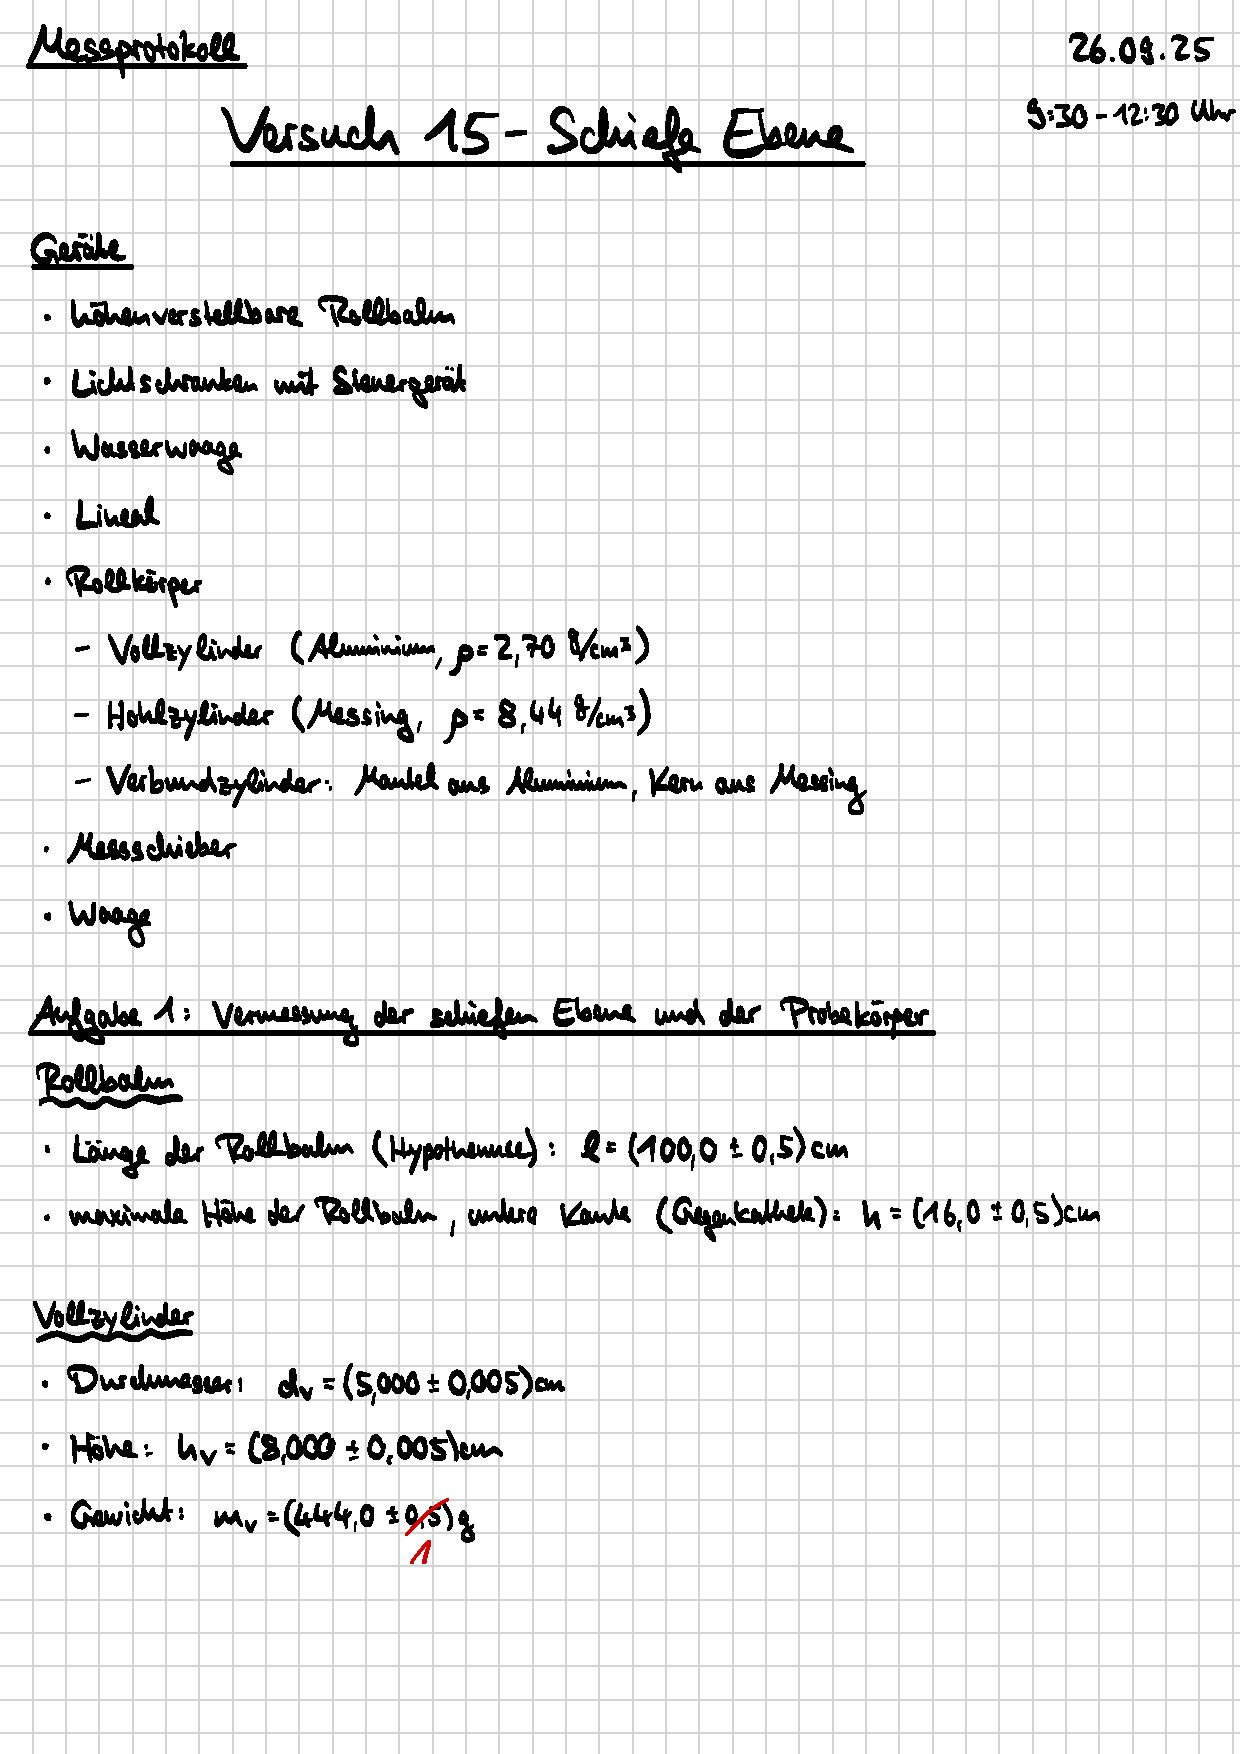
\includegraphics[page=1, width=.95\textwidth,]{PAP1_15_Messprotokoll 2.pdf}
    \caption{Messprotokoll Versuch 15 Seite 1}
\end{figure}
\clearpage
\newpage
\begin{figure}[h!]
    \centering
    \includegraphics[page=2, width=1\textwidth,]{PAP1_15_Messprotokoll 2.pdf}
    \caption{Messprotokoll Versuch 15 Seite 2}
\end{figure}
\newpage
\begin{figure}[h!]
    \centering
    \includegraphics[page=3, width=1\textwidth,]{PAP1_15_Messprotokoll 2.pdf}
    \caption{Messprotokoll Versuch 15  Seite 3}
\end{figure}
\newpage
\begin{figure}[h!]
    \centering
    \includegraphics[page=4, width=0.95\textwidth,]{PAP1_15_Messprotokoll 2.pdf}
    \caption{Messprotokoll Versuch 15 Seite 4}
\end{figure}
\newpage
\begin{figure}[h!]
    \centering
    \includegraphics[page=5, width=1\textwidth,]{PAP1_15_Messprotokoll 2.pdf}
    \caption{Messprotokoll Versuch 15  Seite 5}
\end{figure}
\newpage
\begin{figure}[h!]
    \centering
    \includegraphics[page=6, width=0.95\textwidth,]{PAP1_15_Messprotokoll 2.pdf}
    \caption{Messprotokoll Versuch 15 Seite 6}
\end{figure}
\newpage